\documentclass[twoside]{book}

% Packages required by doxygen
\usepackage{fixltx2e}
\usepackage{calc}
\usepackage{doxygen}
\usepackage[export]{adjustbox} % also loads graphicx
\usepackage{graphicx}
\usepackage[utf8]{inputenc}
\usepackage{makeidx}
\usepackage{multicol}
\usepackage{multirow}
\PassOptionsToPackage{warn}{textcomp}
\usepackage{textcomp}
\usepackage[nointegrals]{wasysym}
\usepackage[table]{xcolor}

% Font selection
\usepackage[T1]{fontenc}
\usepackage[scaled=.90]{helvet}
\usepackage{courier}
\usepackage{amssymb}
\usepackage{sectsty}
\renewcommand{\familydefault}{\sfdefault}
\allsectionsfont{%
  \fontseries{bc}\selectfont%
  \color{darkgray}%
}
\renewcommand{\DoxyLabelFont}{%
  \fontseries{bc}\selectfont%
  \color{darkgray}%
}
\newcommand{\+}{\discretionary{\mbox{\scriptsize$\hookleftarrow$}}{}{}}

% Page & text layout
\usepackage{geometry}
\geometry{%
  a4paper,%
  top=2.5cm,%
  bottom=2.5cm,%
  left=2.5cm,%
  right=2.5cm%
}
\tolerance=750
\hfuzz=15pt
\hbadness=750
\setlength{\emergencystretch}{15pt}
\setlength{\parindent}{0cm}
\setlength{\parskip}{3ex plus 2ex minus 2ex}
\makeatletter
\renewcommand{\paragraph}{%
  \@startsection{paragraph}{4}{0ex}{-1.0ex}{1.0ex}{%
    \normalfont\normalsize\bfseries\SS@parafont%
  }%
}
\renewcommand{\subparagraph}{%
  \@startsection{subparagraph}{5}{0ex}{-1.0ex}{1.0ex}{%
    \normalfont\normalsize\bfseries\SS@subparafont%
  }%
}
\makeatother

% Headers & footers
\usepackage{fancyhdr}
\pagestyle{fancyplain}
\fancyhead[LE]{\fancyplain{}{\bfseries\thepage}}
\fancyhead[CE]{\fancyplain{}{}}
\fancyhead[RE]{\fancyplain{}{\bfseries\leftmark}}
\fancyhead[LO]{\fancyplain{}{\bfseries\rightmark}}
\fancyhead[CO]{\fancyplain{}{}}
\fancyhead[RO]{\fancyplain{}{\bfseries\thepage}}
\fancyfoot[LE]{\fancyplain{}{}}
\fancyfoot[CE]{\fancyplain{}{}}
\fancyfoot[RE]{\fancyplain{}{\bfseries\scriptsize Generated by Doxygen }}
\fancyfoot[LO]{\fancyplain{}{\bfseries\scriptsize Generated by Doxygen }}
\fancyfoot[CO]{\fancyplain{}{}}
\fancyfoot[RO]{\fancyplain{}{}}
\renewcommand{\footrulewidth}{0.4pt}
\renewcommand{\chaptermark}[1]{%
  \markboth{#1}{}%
}
\renewcommand{\sectionmark}[1]{%
  \markright{\thesection\ #1}%
}

% Indices & bibliography
\usepackage{natbib}
\usepackage[titles]{tocloft}
\setcounter{tocdepth}{3}
\setcounter{secnumdepth}{5}
\makeindex

% Hyperlinks (required, but should be loaded last)
\usepackage{ifpdf}
\ifpdf
  \usepackage[pdftex,pagebackref=true]{hyperref}
\else
  \usepackage[ps2pdf,pagebackref=true]{hyperref}
\fi
\hypersetup{%
  colorlinks=true,%
  linkcolor=blue,%
  citecolor=blue,%
  unicode%
}

% Custom commands
\newcommand{\clearemptydoublepage}{%
  \newpage{\pagestyle{empty}\cleardoublepage}%
}

\usepackage{caption}
\captionsetup{labelsep=space,justification=centering,font={bf},singlelinecheck=off,skip=4pt,position=top}

%===== C O N T E N T S =====

\begin{document}

% Titlepage & ToC
\hypersetup{pageanchor=false,
             bookmarksnumbered=true,
             pdfencoding=unicode
            }
\pagenumbering{roman}
\begin{titlepage}
\vspace*{7cm}
\begin{center}%
{\Large My Project }\\
\vspace*{1cm}
{\large Generated by Doxygen 1.8.11}\\
\end{center}
\end{titlepage}
\clearemptydoublepage
\tableofcontents
\clearemptydoublepage
\pagenumbering{arabic}
\hypersetup{pageanchor=true}

%--- Begin generated contents ---
\chapter{Hierarchical Index}
\section{Class Hierarchy}
This inheritance list is sorted roughly, but not completely, alphabetically\+:\begin{DoxyCompactList}
\item binary\+\_\+function\begin{DoxyCompactList}
\item \contentsline{section}{Search}{\pageref{class_search}}{}
\begin{DoxyCompactList}
\item \contentsline{section}{binary\+Search}{\pageref{classbinary_search}}{}
\item \contentsline{section}{linear\+Search}{\pageref{classlinear_search}}{}
\item \contentsline{section}{S\+T\+L\+Search}{\pageref{class_s_t_l_search}}{}
\end{DoxyCompactList}
\end{DoxyCompactList}
\item \contentsline{section}{Test\+Vector}{\pageref{class_test_vector}}{}
\item \contentsline{section}{Timer}{\pageref{class_timer}}{}
\end{DoxyCompactList}

\chapter{Class Index}
\section{Class List}
Here are the classes, structs, unions and interfaces with brief descriptions\+:\begin{DoxyCompactList}
\item\contentsline{section}{\hyperlink{classbinary_search}{binary\+Search} }{\pageref{classbinary_search}}{}
\item\contentsline{section}{\hyperlink{classlinear_search}{linear\+Search} }{\pageref{classlinear_search}}{}
\item\contentsline{section}{\hyperlink{class_search}{Search} }{\pageref{class_search}}{}
\item\contentsline{section}{\hyperlink{class_s_t_l_search}{S\+T\+L\+Search} }{\pageref{class_s_t_l_search}}{}
\item\contentsline{section}{\hyperlink{class_test_vector}{Test\+Vector} }{\pageref{class_test_vector}}{}
\item\contentsline{section}{\hyperlink{class_timer}{Timer} }{\pageref{class_timer}}{}
\end{DoxyCompactList}

\chapter{File Index}
\section{File List}
Here is a list of all files with brief descriptions\+:\begin{DoxyCompactList}
\item\contentsline{section}{\hyperlink{config_8h}{config.\+h} }{\pageref{config_8h}}{}
\item\contentsline{section}{\hyperlink{constructor_8cpp}{constructor.\+cpp} }{\pageref{constructor_8cpp}}{}
\item\contentsline{section}{\hyperlink{inc_8cpp}{inc.\+cpp} }{\pageref{inc_8cpp}}{}
\item\contentsline{section}{\hyperlink{search_8cpp}{search.\+cpp} }{\pageref{search_8cpp}}{}
\item\contentsline{section}{\hyperlink{sort_8cpp}{sort.\+cpp} }{\pageref{sort_8cpp}}{}
\item\contentsline{section}{\hyperlink{test13_8cpp}{test13.\+cpp} }{\pageref{test13_8cpp}}{}
\item\contentsline{section}{\hyperlink{testtimer_8cpp}{testtimer.\+cpp} }{\pageref{testtimer_8cpp}}{}
\item\contentsline{section}{\hyperlink{testvector_8cpp}{testvector.\+cpp} }{\pageref{testvector_8cpp}}{}
\item\contentsline{section}{\hyperlink{testvector_8h}{testvector.\+h} }{\pageref{testvector_8h}}{}
\item\contentsline{section}{\hyperlink{_timer_8cpp}{Timer.\+cpp} }{\pageref{_timer_8cpp}}{}
\item\contentsline{section}{\hyperlink{_timer_8h}{Timer.\+h} }{\pageref{_timer_8h}}{}
\end{DoxyCompactList}

\chapter{Class Documentation}
\hypertarget{classbinary_search}{}\section{binary\+Search Class Reference}
\label{classbinary_search}\index{binary\+Search@{binary\+Search}}
Inheritance diagram for binary\+Search\+:\begin{figure}[H]
\begin{center}
\leavevmode
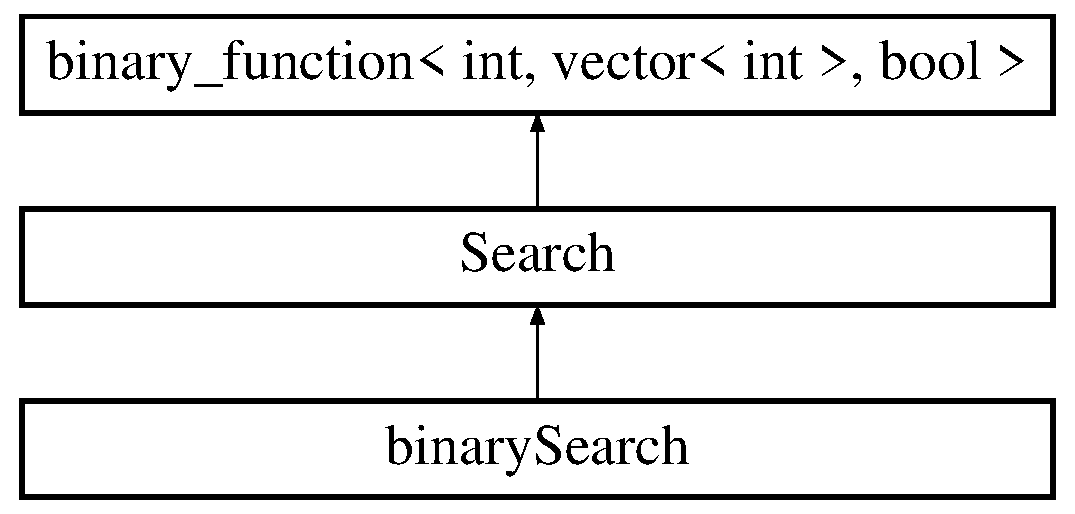
\includegraphics[height=3.000000cm]{classbinary_search}
\end{center}
\end{figure}
\subsection*{Public Member Functions}
\begin{DoxyCompactItemize}
\item 
bool \hyperlink{classbinary_search_a8e145edfb29183d7e1b265bd4cf4293f}{operator()} (int search\+Value, const vector$<$ int $>$ \&keys) const 
\end{DoxyCompactItemize}


\subsection{Member Function Documentation}
\index{binary\+Search@{binary\+Search}!operator()@{operator()}}
\index{operator()@{operator()}!binary\+Search@{binary\+Search}}
\subsubsection[{\texorpdfstring{operator()(int search\+Value, const vector$<$ int $>$ \&keys) const }{operator()(int searchValue, const vector< int > &keys) const }}]{\setlength{\rightskip}{0pt plus 5cm}bool binary\+Search\+::operator() (
\begin{DoxyParamCaption}
\item[{int}]{search\+Value, }
\item[{const vector$<$ int $>$ \&}]{keys}
\end{DoxyParamCaption}
) const\hspace{0.3cm}{\ttfamily [inline]}, {\ttfamily [virtual]}}\hypertarget{classbinary_search_a8e145edfb29183d7e1b265bd4cf4293f}{}\label{classbinary_search_a8e145edfb29183d7e1b265bd4cf4293f}


Implements \hyperlink{class_search}{Search}.



The documentation for this class was generated from the following file\+:\begin{DoxyCompactItemize}
\item 
\hyperlink{search_8cpp}{search.\+cpp}\end{DoxyCompactItemize}

\hypertarget{classlinear_search}{}\section{linear\+Search Class Reference}
\label{classlinear_search}\index{linear\+Search@{linear\+Search}}
Inheritance diagram for linear\+Search\+:\begin{figure}[H]
\begin{center}
\leavevmode
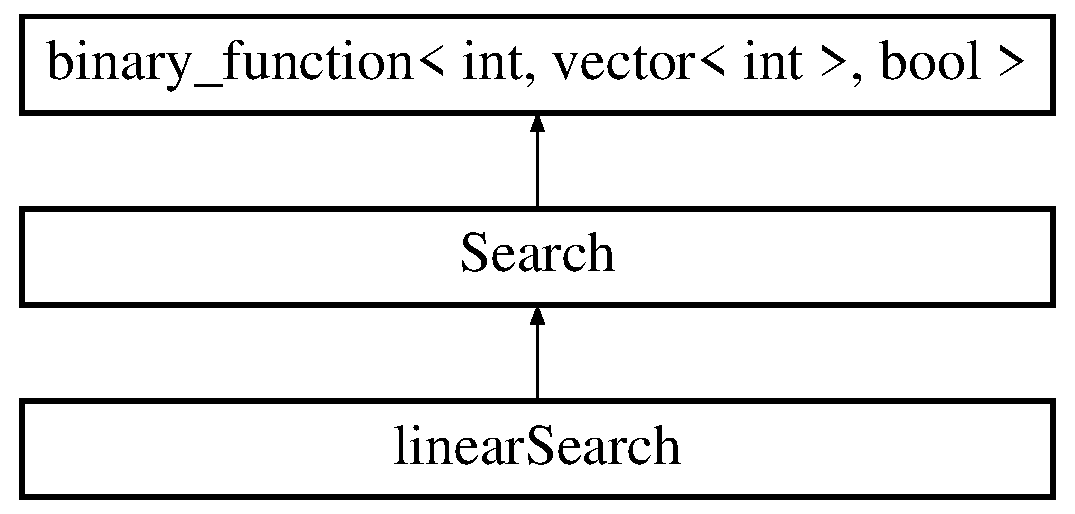
\includegraphics[height=3.000000cm]{classlinear_search}
\end{center}
\end{figure}
\subsection*{Public Member Functions}
\begin{DoxyCompactItemize}
\item 
bool \hyperlink{classlinear_search_a447bc4f724457f1786dc36c10626bfa8}{operator()} (int search\+Value, const vector$<$ int $>$ \&keys) const 
\end{DoxyCompactItemize}


\subsection{Member Function Documentation}
\index{linear\+Search@{linear\+Search}!operator()@{operator()}}
\index{operator()@{operator()}!linear\+Search@{linear\+Search}}
\subsubsection[{\texorpdfstring{operator()(int search\+Value, const vector$<$ int $>$ \&keys) const }{operator()(int searchValue, const vector< int > &keys) const }}]{\setlength{\rightskip}{0pt plus 5cm}bool linear\+Search\+::operator() (
\begin{DoxyParamCaption}
\item[{int}]{search\+Value, }
\item[{const vector$<$ int $>$ \&}]{keys}
\end{DoxyParamCaption}
) const\hspace{0.3cm}{\ttfamily [inline]}, {\ttfamily [virtual]}}\hypertarget{classlinear_search_a447bc4f724457f1786dc36c10626bfa8}{}\label{classlinear_search_a447bc4f724457f1786dc36c10626bfa8}


Implements \hyperlink{class_search}{Search}.



The documentation for this class was generated from the following file\+:\begin{DoxyCompactItemize}
\item 
\hyperlink{search_8cpp}{search.\+cpp}\end{DoxyCompactItemize}

\hypertarget{class_search}{}\section{Search Class Reference}
\label{class_search}\index{Search@{Search}}
Inheritance diagram for Search\+:\begin{figure}[H]
\begin{center}
\leavevmode
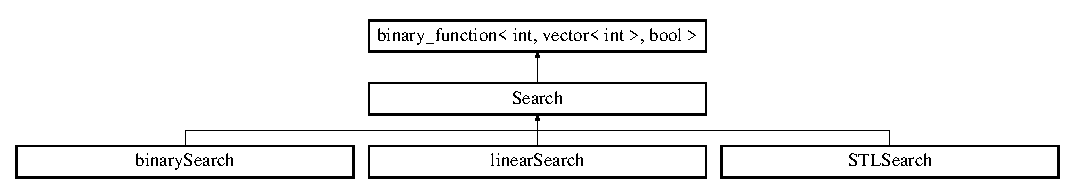
\includegraphics[height=2.153846cm]{class_search}
\end{center}
\end{figure}


The documentation for this class was generated from the following file\+:\begin{DoxyCompactItemize}
\item 
\hyperlink{search_8cpp}{search.\+cpp}\end{DoxyCompactItemize}

\hypertarget{class_s_t_l_search}{}\section{S\+T\+L\+Search Class Reference}
\label{class_s_t_l_search}\index{S\+T\+L\+Search@{S\+T\+L\+Search}}
Inheritance diagram for S\+T\+L\+Search\+:\begin{figure}[H]
\begin{center}
\leavevmode
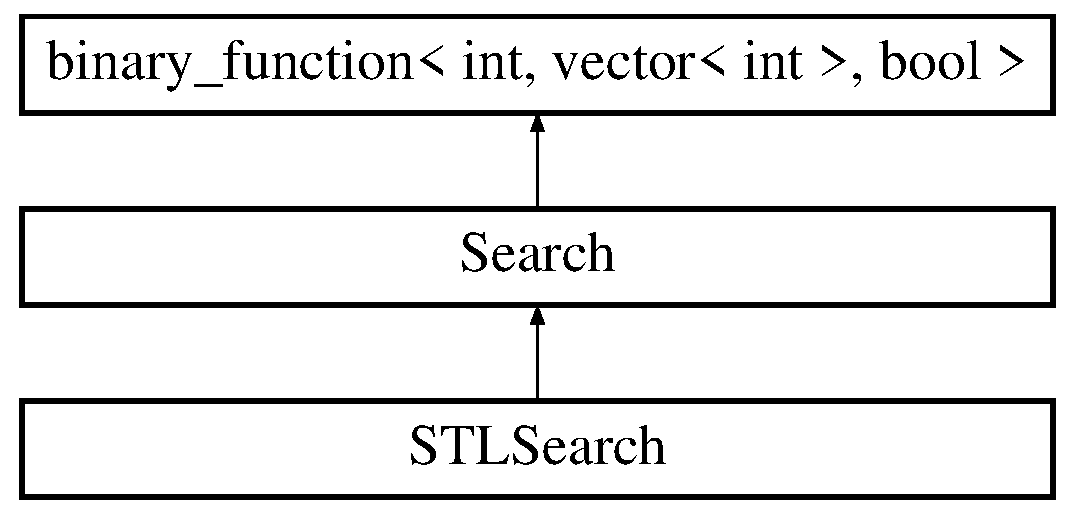
\includegraphics[height=3.000000cm]{class_s_t_l_search}
\end{center}
\end{figure}
\subsection*{Public Member Functions}
\begin{DoxyCompactItemize}
\item 
bool \hyperlink{class_s_t_l_search_a0f3684e33bd5e47317ab5a94d6f52dba}{operator()} (int search\+Value, const vector$<$ int $>$ \&keys) const 
\end{DoxyCompactItemize}


\subsection{Member Function Documentation}
\index{S\+T\+L\+Search@{S\+T\+L\+Search}!operator()@{operator()}}
\index{operator()@{operator()}!S\+T\+L\+Search@{S\+T\+L\+Search}}
\subsubsection[{\texorpdfstring{operator()(int search\+Value, const vector$<$ int $>$ \&keys) const }{operator()(int searchValue, const vector< int > &keys) const }}]{\setlength{\rightskip}{0pt plus 5cm}bool S\+T\+L\+Search\+::operator() (
\begin{DoxyParamCaption}
\item[{int}]{search\+Value, }
\item[{const vector$<$ int $>$ \&}]{keys}
\end{DoxyParamCaption}
) const\hspace{0.3cm}{\ttfamily [inline]}, {\ttfamily [virtual]}}\hypertarget{class_s_t_l_search_a0f3684e33bd5e47317ab5a94d6f52dba}{}\label{class_s_t_l_search_a0f3684e33bd5e47317ab5a94d6f52dba}


Implements \hyperlink{class_search}{Search}.



The documentation for this class was generated from the following file\+:\begin{DoxyCompactItemize}
\item 
\hyperlink{search_8cpp}{search.\+cpp}\end{DoxyCompactItemize}

\hypertarget{class_test_vector}{}\section{Test\+Vector Class Reference}
\label{class_test_vector}\index{Test\+Vector@{Test\+Vector}}


{\ttfamily \#include $<$testvector.\+h$>$}

\subsection*{Public Member Functions}
\begin{DoxyCompactItemize}
\item 
\hyperlink{class_test_vector_abf540180761043bb7ac2665e147bdd33}{Test\+Vector} (int size)
\item 
\hyperlink{class_test_vector_a4a48046f67cc822ce9a6907f022a5d61}{Test\+Vector} (const \hyperlink{class_test_vector}{Test\+Vector} \&rhs)
\item 
\hyperlink{class_test_vector}{Test\+Vector} \& \hyperlink{class_test_vector_a8d4a95de7e0e9985ffcd86280efb631d}{operator++} ()
\item 
\hyperlink{class_test_vector}{Test\+Vector} \hyperlink{class_test_vector_a1b9640623055cd4618606cd2f0ed08b3}{operator++} (int ignored)
\item 
int \hyperlink{class_test_vector_ae244371b88cb0ab127a877e5206b7ed8}{operator\mbox{[}$\,$\mbox{]}} (int loc) const 
\end{DoxyCompactItemize}


\subsection{Constructor \& Destructor Documentation}
\index{Test\+Vector@{Test\+Vector}!Test\+Vector@{Test\+Vector}}
\index{Test\+Vector@{Test\+Vector}!Test\+Vector@{Test\+Vector}}
\subsubsection[{\texorpdfstring{Test\+Vector(int size)}{TestVector(int size)}}]{\setlength{\rightskip}{0pt plus 5cm}Test\+Vector\+::\+Test\+Vector (
\begin{DoxyParamCaption}
\item[{int}]{size}
\end{DoxyParamCaption}
)}\hypertarget{class_test_vector_abf540180761043bb7ac2665e147bdd33}{}\label{class_test_vector_abf540180761043bb7ac2665e147bdd33}
\index{Test\+Vector@{Test\+Vector}!Test\+Vector@{Test\+Vector}}
\index{Test\+Vector@{Test\+Vector}!Test\+Vector@{Test\+Vector}}
\subsubsection[{\texorpdfstring{Test\+Vector(const Test\+Vector \&rhs)}{TestVector(const TestVector &rhs)}}]{\setlength{\rightskip}{0pt plus 5cm}Test\+Vector\+::\+Test\+Vector (
\begin{DoxyParamCaption}
\item[{const {\bf Test\+Vector} \&}]{rhs}
\end{DoxyParamCaption}
)}\hypertarget{class_test_vector_a4a48046f67cc822ce9a6907f022a5d61}{}\label{class_test_vector_a4a48046f67cc822ce9a6907f022a5d61}


\subsection{Member Function Documentation}
\index{Test\+Vector@{Test\+Vector}!operator++@{operator++}}
\index{operator++@{operator++}!Test\+Vector@{Test\+Vector}}
\subsubsection[{\texorpdfstring{operator++()}{operator++()}}]{\setlength{\rightskip}{0pt plus 5cm}{\bf Test\+Vector} \& Test\+Vector\+::operator++ (
\begin{DoxyParamCaption}
{}
\end{DoxyParamCaption}
)}\hypertarget{class_test_vector_a8d4a95de7e0e9985ffcd86280efb631d}{}\label{class_test_vector_a8d4a95de7e0e9985ffcd86280efb631d}
\index{Test\+Vector@{Test\+Vector}!operator++@{operator++}}
\index{operator++@{operator++}!Test\+Vector@{Test\+Vector}}
\subsubsection[{\texorpdfstring{operator++(int ignored)}{operator++(int ignored)}}]{\setlength{\rightskip}{0pt plus 5cm}{\bf Test\+Vector} Test\+Vector\+::operator++ (
\begin{DoxyParamCaption}
\item[{int}]{ignored}
\end{DoxyParamCaption}
)}\hypertarget{class_test_vector_a1b9640623055cd4618606cd2f0ed08b3}{}\label{class_test_vector_a1b9640623055cd4618606cd2f0ed08b3}
\index{Test\+Vector@{Test\+Vector}!operator\mbox{[}$\,$\mbox{]}@{operator[]}}
\index{operator\mbox{[}$\,$\mbox{]}@{operator[]}!Test\+Vector@{Test\+Vector}}
\subsubsection[{\texorpdfstring{operator[](int loc) const }{operator[](int loc) const }}]{\setlength{\rightskip}{0pt plus 5cm}int Test\+Vector\+::operator\mbox{[}$\,$\mbox{]} (
\begin{DoxyParamCaption}
\item[{int}]{loc}
\end{DoxyParamCaption}
) const}\hypertarget{class_test_vector_ae244371b88cb0ab127a877e5206b7ed8}{}\label{class_test_vector_ae244371b88cb0ab127a877e5206b7ed8}


The documentation for this class was generated from the following files\+:\begin{DoxyCompactItemize}
\item 
\hyperlink{testvector_8h}{testvector.\+h}\item 
\hyperlink{testvector_8cpp}{testvector.\+cpp}\end{DoxyCompactItemize}

\hypertarget{class_timer}{}\section{Timer Class Reference}
\label{class_timer}\index{Timer@{Timer}}


{\ttfamily \#include $<$Timer.\+h$>$}

\subsection*{Public Member Functions}
\begin{DoxyCompactItemize}
\item 
\hyperlink{class_timer_a5f16e8da27d2a5a5242dead46de05d97}{Timer} ()
\item 
void \hyperlink{class_timer_a3a8b5272198d029779dc9302a54305a8}{start} ()  throw (runtime\+\_\+error)
\item 
void \hyperlink{class_timer_a63f0eb44b27402196590a03781515dba}{stop} ()  throw (logic\+\_\+error)
\item 
double \hyperlink{class_timer_ad306e18f8d8a0296e001683f92d7f86e}{get\+Elapsed\+Time} () const   throw (logic\+\_\+error)
\end{DoxyCompactItemize}


\subsection{Constructor \& Destructor Documentation}
\index{Timer@{Timer}!Timer@{Timer}}
\index{Timer@{Timer}!Timer@{Timer}}
\subsubsection[{\texorpdfstring{Timer()}{Timer()}}]{\setlength{\rightskip}{0pt plus 5cm}Timer\+::\+Timer (
\begin{DoxyParamCaption}
{}
\end{DoxyParamCaption}
)}\hypertarget{class_timer_a5f16e8da27d2a5a5242dead46de05d97}{}\label{class_timer_a5f16e8da27d2a5a5242dead46de05d97}
Constructor that intializes timer\+Was\+Started to false and begin time and duration to -\/1 to indicate that the clock has not read time yet

\begin{DoxyReturn}{Returns}
constructor
\end{DoxyReturn}
\begin{DoxyPrecond}{Precondition}
unitialized timer object 
\end{DoxyPrecond}
\begin{DoxyPostcond}{Postcondition}
an initialized timer object with beging time and end time being -\/1 to indicate stopped 
\end{DoxyPostcond}


\subsection{Member Function Documentation}
\index{Timer@{Timer}!get\+Elapsed\+Time@{get\+Elapsed\+Time}}
\index{get\+Elapsed\+Time@{get\+Elapsed\+Time}!Timer@{Timer}}
\subsubsection[{\texorpdfstring{get\+Elapsed\+Time() const }{getElapsedTime() const }}]{\setlength{\rightskip}{0pt plus 5cm}double Timer\+::get\+Elapsed\+Time (
\begin{DoxyParamCaption}
{}
\end{DoxyParamCaption}
) const throw  logic\+\_\+error) }\hypertarget{class_timer_ad306e18f8d8a0296e001683f92d7f86e}{}\label{class_timer_ad306e18f8d8a0296e001683f92d7f86e}
Get\+Elapsed\+Time method that uses the begin\+Time and duration to calculate the amount of time that has passed

\begin{DoxyReturn}{Returns}
double that is duration -\/ begin\+Time
\end{DoxyReturn}
\begin{DoxyPrecond}{Precondition}
two timevals indicating the start and end of an interval
\end{DoxyPrecond}
\begin{DoxyPostcond}{Postcondition}
a single double that represents the amount of time passed
\end{DoxyPostcond}

\begin{DoxyExceptions}{Exceptions}
{\em throws} & logic error if either of the timevals have not been set \\
\hline
\end{DoxyExceptions}
\index{Timer@{Timer}!start@{start}}
\index{start@{start}!Timer@{Timer}}
\subsubsection[{\texorpdfstring{start()}{start()}}]{\setlength{\rightskip}{0pt plus 5cm}void Timer\+::start (
\begin{DoxyParamCaption}
{}
\end{DoxyParamCaption}
) throw  runtime\+\_\+error) }\hypertarget{class_timer_a3a8b5272198d029779dc9302a54305a8}{}\label{class_timer_a3a8b5272198d029779dc9302a54305a8}
Start method that starts the timer by calling gettimeofday() and sets timer\+Was\+Started to true

\begin{DoxyReturn}{Returns}
void
\end{DoxyReturn}
\begin{DoxyPrecond}{Precondition}
unstarted timer and timer\+Was\+Started is false
\end{DoxyPrecond}
\begin{DoxyPostcond}{Postcondition}
timer is started and begin time has been set as well as timer\+Was\+Started (true)
\end{DoxyPostcond}

\begin{DoxyExceptions}{Exceptions}
{\em throws} & runtime error if gettimeofday does not set the time \\
\hline
\end{DoxyExceptions}
\index{Timer@{Timer}!stop@{stop}}
\index{stop@{stop}!Timer@{Timer}}
\subsubsection[{\texorpdfstring{stop()}{stop()}}]{\setlength{\rightskip}{0pt plus 5cm}void Timer\+::stop (
\begin{DoxyParamCaption}
{}
\end{DoxyParamCaption}
) throw  logic\+\_\+error) }\hypertarget{class_timer_a63f0eb44b27402196590a03781515dba}{}\label{class_timer_a63f0eb44b27402196590a03781515dba}
Stop method that stops the timer by calling gettimeofday() and sets timer\+Was\+Started to false

\begin{DoxyReturn}{Returns}
void
\end{DoxyReturn}
\begin{DoxyPrecond}{Precondition}
started timer and timer\+Was\+Started is true
\end{DoxyPrecond}
\begin{DoxyPostcond}{Postcondition}
timer is stopped and stopped has been set as well as timer\+Was\+Started (false)
\end{DoxyPostcond}

\begin{DoxyExceptions}{Exceptions}
{\em throws} & logic error an attempt to stop the timer is made prior to starting the timer \\
\hline
\end{DoxyExceptions}


The documentation for this class was generated from the following files\+:\begin{DoxyCompactItemize}
\item 
\hyperlink{_timer_8h}{Timer.\+h}\item 
\hyperlink{_timer_8cpp}{Timer.\+cpp}\end{DoxyCompactItemize}

\chapter{File Documentation}
\hypertarget{config_8h}{}\section{config.\+h File Reference}
\label{config_8h}\index{config.\+h@{config.\+h}}
\subsection*{Macros}
\begin{DoxyCompactItemize}
\item 
\#define \hyperlink{config_8h_a0e3bcdcc18baaef148831f8a291d2390}{L\+A\+B13\+\_\+\+T\+E\+S\+T1}~0
\item 
\#define \hyperlink{config_8h_a4a01327c2af4e3d5f89681a79776b319}{L\+A\+B13\+\_\+\+T\+E\+S\+T2}~0
\end{DoxyCompactItemize}


\subsection{Macro Definition Documentation}
\index{config.\+h@{config.\+h}!L\+A\+B13\+\_\+\+T\+E\+S\+T1@{L\+A\+B13\+\_\+\+T\+E\+S\+T1}}
\index{L\+A\+B13\+\_\+\+T\+E\+S\+T1@{L\+A\+B13\+\_\+\+T\+E\+S\+T1}!config.\+h@{config.\+h}}
\subsubsection[{\texorpdfstring{L\+A\+B13\+\_\+\+T\+E\+S\+T1}{LAB13_TEST1}}]{\setlength{\rightskip}{0pt plus 5cm}\#define L\+A\+B13\+\_\+\+T\+E\+S\+T1~0}\hypertarget{config_8h_a0e3bcdcc18baaef148831f8a291d2390}{}\label{config_8h_a0e3bcdcc18baaef148831f8a291d2390}
\hyperlink{class_timer}{Timer} class (Lab 13) configuration file. Activate test \textquotesingle{}N\textquotesingle{} by defining the corresponding L\+A\+B12\+\_\+\+T\+E\+S\+TN to have the value 1. \index{config.\+h@{config.\+h}!L\+A\+B13\+\_\+\+T\+E\+S\+T2@{L\+A\+B13\+\_\+\+T\+E\+S\+T2}}
\index{L\+A\+B13\+\_\+\+T\+E\+S\+T2@{L\+A\+B13\+\_\+\+T\+E\+S\+T2}!config.\+h@{config.\+h}}
\subsubsection[{\texorpdfstring{L\+A\+B13\+\_\+\+T\+E\+S\+T2}{LAB13_TEST2}}]{\setlength{\rightskip}{0pt plus 5cm}\#define L\+A\+B13\+\_\+\+T\+E\+S\+T2~0}\hypertarget{config_8h_a4a01327c2af4e3d5f89681a79776b319}{}\label{config_8h_a4a01327c2af4e3d5f89681a79776b319}

\hypertarget{constructor_8cpp}{}\section{constructor.\+cpp File Reference}
\label{constructor_8cpp}\index{constructor.\+cpp@{constructor.\+cpp}}
{\ttfamily \#include $<$iostream$>$}\\*
{\ttfamily \#include $<$string$>$}\\*
{\ttfamily \#include \char`\"{}Timer.\+h\char`\"{}}\\*
{\ttfamily \#include \char`\"{}Test\+Vector.\+h\char`\"{}}\\*
\subsection*{Macros}
\begin{DoxyCompactItemize}
\item 
\#define \hyperlink{constructor_8cpp_a68628a242ca66ca281565d52838cfe5a}{run\+Test}(Type)~\hyperlink{constructor_8cpp_ad22cbf7b1a579c4ab9c44ad7c5702307}{test\+Constructor}$<$Type$>$(num\+Values, \#Type)
\end{DoxyCompactItemize}
\subsection*{Functions}
\begin{DoxyCompactItemize}
\item 
{\footnotesize template$<$typename Data\+Type $>$ }\\int \hyperlink{constructor_8cpp_a4b2651e00b4a1a56d4bede535326e183}{test\+Compute} (Data\+Type value)
\item 
{\footnotesize template$<$$>$ }\\int \hyperlink{constructor_8cpp_a598f26df9f699feec4990601add252ea}{test\+Compute$<$ int $>$} (int value)
\item 
{\footnotesize template$<$$>$ }\\int \hyperlink{constructor_8cpp_ae9df768a369700534cc9f7fc43b1d043}{test\+Compute$<$ double $>$} (double value)
\item 
{\footnotesize template$<$typename Data\+Type $>$ }\\void \hyperlink{constructor_8cpp_ad22cbf7b1a579c4ab9c44ad7c5702307}{test\+Constructor} (int num\+Values, string name)
\item 
int \hyperlink{constructor_8cpp_a3c04138a5bfe5d72780bb7e82a18e627}{main} (int argc, char $\ast$$\ast$argv)
\end{DoxyCompactItemize}
\subsection*{Variables}
\begin{DoxyCompactItemize}
\item 
const int \hyperlink{constructor_8cpp_a1718f5513e9597ba62d1fcedeafec0c1}{num\+Repetitions} = 1000000
\end{DoxyCompactItemize}


\subsection{Macro Definition Documentation}
\index{constructor.\+cpp@{constructor.\+cpp}!run\+Test@{run\+Test}}
\index{run\+Test@{run\+Test}!constructor.\+cpp@{constructor.\+cpp}}
\subsubsection[{\texorpdfstring{run\+Test}{runTest}}]{\setlength{\rightskip}{0pt plus 5cm}\#define run\+Test(
\begin{DoxyParamCaption}
\item[{}]{Type}
\end{DoxyParamCaption}
)~{\bf test\+Constructor}$<$Type$>$(num\+Values, \#Type)}\hypertarget{constructor_8cpp_a68628a242ca66ca281565d52838cfe5a}{}\label{constructor_8cpp_a68628a242ca66ca281565d52838cfe5a}


\subsection{Function Documentation}
\index{constructor.\+cpp@{constructor.\+cpp}!main@{main}}
\index{main@{main}!constructor.\+cpp@{constructor.\+cpp}}
\subsubsection[{\texorpdfstring{main(int argc, char $\ast$$\ast$argv)}{main(int argc, char **argv)}}]{\setlength{\rightskip}{0pt plus 5cm}int main (
\begin{DoxyParamCaption}
\item[{int}]{argc, }
\item[{char $\ast$$\ast$}]{argv}
\end{DoxyParamCaption}
)}\hypertarget{constructor_8cpp_a3c04138a5bfe5d72780bb7e82a18e627}{}\label{constructor_8cpp_a3c04138a5bfe5d72780bb7e82a18e627}
\index{constructor.\+cpp@{constructor.\+cpp}!test\+Compute@{test\+Compute}}
\index{test\+Compute@{test\+Compute}!constructor.\+cpp@{constructor.\+cpp}}
\subsubsection[{\texorpdfstring{test\+Compute(\+Data\+Type value)}{testCompute(DataType value)}}]{\setlength{\rightskip}{0pt plus 5cm}template$<$typename Data\+Type $>$ int test\+Compute (
\begin{DoxyParamCaption}
\item[{Data\+Type}]{value}
\end{DoxyParamCaption}
)}\hypertarget{constructor_8cpp_a4b2651e00b4a1a56d4bede535326e183}{}\label{constructor_8cpp_a4b2651e00b4a1a56d4bede535326e183}
\index{constructor.\+cpp@{constructor.\+cpp}!test\+Compute$<$ double $>$@{test\+Compute$<$ double $>$}}
\index{test\+Compute$<$ double $>$@{test\+Compute$<$ double $>$}!constructor.\+cpp@{constructor.\+cpp}}
\subsubsection[{\texorpdfstring{test\+Compute$<$ double $>$(double value)}{testCompute< double >(double value)}}]{\setlength{\rightskip}{0pt plus 5cm}template$<$$>$ int {\bf test\+Compute}$<$ double $>$ (
\begin{DoxyParamCaption}
\item[{double}]{value}
\end{DoxyParamCaption}
)}\hypertarget{constructor_8cpp_ae9df768a369700534cc9f7fc43b1d043}{}\label{constructor_8cpp_ae9df768a369700534cc9f7fc43b1d043}
\index{constructor.\+cpp@{constructor.\+cpp}!test\+Compute$<$ int $>$@{test\+Compute$<$ int $>$}}
\index{test\+Compute$<$ int $>$@{test\+Compute$<$ int $>$}!constructor.\+cpp@{constructor.\+cpp}}
\subsubsection[{\texorpdfstring{test\+Compute$<$ int $>$(int value)}{testCompute< int >(int value)}}]{\setlength{\rightskip}{0pt plus 5cm}template$<$$>$ int {\bf test\+Compute}$<$ int $>$ (
\begin{DoxyParamCaption}
\item[{int}]{value}
\end{DoxyParamCaption}
)}\hypertarget{constructor_8cpp_a598f26df9f699feec4990601add252ea}{}\label{constructor_8cpp_a598f26df9f699feec4990601add252ea}
\index{constructor.\+cpp@{constructor.\+cpp}!test\+Constructor@{test\+Constructor}}
\index{test\+Constructor@{test\+Constructor}!constructor.\+cpp@{constructor.\+cpp}}
\subsubsection[{\texorpdfstring{test\+Constructor(int num\+Values, string name)}{testConstructor(int numValues, string name)}}]{\setlength{\rightskip}{0pt plus 5cm}template$<$typename Data\+Type $>$ void test\+Constructor (
\begin{DoxyParamCaption}
\item[{int}]{num\+Values, }
\item[{string}]{name}
\end{DoxyParamCaption}
)}\hypertarget{constructor_8cpp_ad22cbf7b1a579c4ab9c44ad7c5702307}{}\label{constructor_8cpp_ad22cbf7b1a579c4ab9c44ad7c5702307}


\subsection{Variable Documentation}
\index{constructor.\+cpp@{constructor.\+cpp}!num\+Repetitions@{num\+Repetitions}}
\index{num\+Repetitions@{num\+Repetitions}!constructor.\+cpp@{constructor.\+cpp}}
\subsubsection[{\texorpdfstring{num\+Repetitions}{numRepetitions}}]{\setlength{\rightskip}{0pt plus 5cm}const int num\+Repetitions = 1000000}\hypertarget{constructor_8cpp_a1718f5513e9597ba62d1fcedeafec0c1}{}\label{constructor_8cpp_a1718f5513e9597ba62d1fcedeafec0c1}

\hypertarget{inc_8cpp}{}\section{inc.\+cpp File Reference}
\label{inc_8cpp}\index{inc.\+cpp@{inc.\+cpp}}
{\ttfamily \#include $<$iostream$>$}\\*
{\ttfamily \#include \char`\"{}Timer.\+h\char`\"{}}\\*
{\ttfamily \#include \char`\"{}Test\+Vector.\+h\char`\"{}}\\*
\subsection*{Functions}
\begin{DoxyCompactItemize}
\item 
int \hyperlink{inc_8cpp_a3c04138a5bfe5d72780bb7e82a18e627}{main} (int argc, char $\ast$$\ast$argv)
\end{DoxyCompactItemize}
\subsection*{Variables}
\begin{DoxyCompactItemize}
\item 
const int \hyperlink{inc_8cpp_a1718f5513e9597ba62d1fcedeafec0c1}{num\+Repetitions} = 1000000
\end{DoxyCompactItemize}


\subsection{Function Documentation}
\index{inc.\+cpp@{inc.\+cpp}!main@{main}}
\index{main@{main}!inc.\+cpp@{inc.\+cpp}}
\subsubsection[{\texorpdfstring{main(int argc, char $\ast$$\ast$argv)}{main(int argc, char **argv)}}]{\setlength{\rightskip}{0pt plus 5cm}int main (
\begin{DoxyParamCaption}
\item[{int}]{argc, }
\item[{char $\ast$$\ast$}]{argv}
\end{DoxyParamCaption}
)}\hypertarget{inc_8cpp_a3c04138a5bfe5d72780bb7e82a18e627}{}\label{inc_8cpp_a3c04138a5bfe5d72780bb7e82a18e627}


\subsection{Variable Documentation}
\index{inc.\+cpp@{inc.\+cpp}!num\+Repetitions@{num\+Repetitions}}
\index{num\+Repetitions@{num\+Repetitions}!inc.\+cpp@{inc.\+cpp}}
\subsubsection[{\texorpdfstring{num\+Repetitions}{numRepetitions}}]{\setlength{\rightskip}{0pt plus 5cm}const int num\+Repetitions = 1000000}\hypertarget{inc_8cpp_a1718f5513e9597ba62d1fcedeafec0c1}{}\label{inc_8cpp_a1718f5513e9597ba62d1fcedeafec0c1}

\hypertarget{search_8cpp}{}\section{search.\+cpp File Reference}
\label{search_8cpp}\index{search.\+cpp@{search.\+cpp}}
{\ttfamily \#include $<$iostream$>$}\\*
{\ttfamily \#include $<$algorithm$>$}\\*
{\ttfamily \#include $<$vector$>$}\\*
{\ttfamily \#include \char`\"{}Timer.\+h\char`\"{}}\\*
\subsection*{Classes}
\begin{DoxyCompactItemize}
\item 
class \hyperlink{class_search}{Search}
\item 
class \hyperlink{classlinear_search}{linear\+Search}
\item 
class \hyperlink{classbinary_search}{binary\+Search}
\item 
class \hyperlink{class_s_t_l_search}{S\+T\+L\+Search}
\end{DoxyCompactItemize}
\subsection*{Functions}
\begin{DoxyCompactItemize}
\item 
int \hyperlink{search_8cpp_a3c04138a5bfe5d72780bb7e82a18e627}{main} (int argc, char $\ast$$\ast$argv)
\end{DoxyCompactItemize}
\subsection*{Variables}
\begin{DoxyCompactItemize}
\item 
const int \hyperlink{search_8cpp_ab57a4f4d64581df58bc7056d4622bd51}{num\+Searches} = 100000
\end{DoxyCompactItemize}


\subsection{Function Documentation}
\index{search.\+cpp@{search.\+cpp}!main@{main}}
\index{main@{main}!search.\+cpp@{search.\+cpp}}
\subsubsection[{\texorpdfstring{main(int argc, char $\ast$$\ast$argv)}{main(int argc, char **argv)}}]{\setlength{\rightskip}{0pt plus 5cm}int main (
\begin{DoxyParamCaption}
\item[{int}]{argc, }
\item[{char $\ast$$\ast$}]{argv}
\end{DoxyParamCaption}
)}\hypertarget{search_8cpp_a3c04138a5bfe5d72780bb7e82a18e627}{}\label{search_8cpp_a3c04138a5bfe5d72780bb7e82a18e627}


\subsection{Variable Documentation}
\index{search.\+cpp@{search.\+cpp}!num\+Searches@{num\+Searches}}
\index{num\+Searches@{num\+Searches}!search.\+cpp@{search.\+cpp}}
\subsubsection[{\texorpdfstring{num\+Searches}{numSearches}}]{\setlength{\rightskip}{0pt plus 5cm}const int num\+Searches = 100000}\hypertarget{search_8cpp_ab57a4f4d64581df58bc7056d4622bd51}{}\label{search_8cpp_ab57a4f4d64581df58bc7056d4622bd51}

\hypertarget{sort_8cpp}{}\section{sort.\+cpp File Reference}
\label{sort_8cpp}\index{sort.\+cpp@{sort.\+cpp}}
{\ttfamily \#include $<$iostream$>$}\\*
{\ttfamily \#include $<$algorithm$>$}\\*
{\ttfamily \#include $<$vector$>$}\\*
{\ttfamily \#include \char`\"{}Timer.\+h\char`\"{}}\\*
\subsection*{Functions}
\begin{DoxyCompactItemize}
\item 
void \hyperlink{sort_8cpp_ac179a0b850c1810c6010e243c052f086}{selection\+Sort} (vector$<$ int $>$\+::iterator front, vector$<$ int $>$\+::iterator back)
\item 
void \hyperlink{sort_8cpp_abbe21f1a370550721fd4eef6aa762b2c}{quick\+Sort} (vector$<$ int $>$\+::iterator front, vector$<$ int $>$\+::iterator back)
\item 
void \hyperlink{sort_8cpp_afefe359fd0c528b6f73b38efda54714b}{time\+Sort} (void($\ast$fcn)(vector$<$ int $>$\+::iterator front, vector$<$ int $>$\+::iterator back), const string name, const vector$<$ int $>$ \&master\+List, const \hyperlink{class_timer}{Timer} \&overhead)
\item 
int \hyperlink{sort_8cpp_a3c04138a5bfe5d72780bb7e82a18e627}{main} (int argc, char $\ast$$\ast$argv)
\end{DoxyCompactItemize}
\subsection*{Variables}
\begin{DoxyCompactItemize}
\item 
const int \hyperlink{sort_8cpp_ad497c97c4b85d09bae6654a1cc2d8899}{num\+Sorts} = 100
\end{DoxyCompactItemize}


\subsection{Function Documentation}
\index{sort.\+cpp@{sort.\+cpp}!main@{main}}
\index{main@{main}!sort.\+cpp@{sort.\+cpp}}
\subsubsection[{\texorpdfstring{main(int argc, char $\ast$$\ast$argv)}{main(int argc, char **argv)}}]{\setlength{\rightskip}{0pt plus 5cm}int main (
\begin{DoxyParamCaption}
\item[{int}]{argc, }
\item[{char $\ast$$\ast$}]{argv}
\end{DoxyParamCaption}
)}\hypertarget{sort_8cpp_a3c04138a5bfe5d72780bb7e82a18e627}{}\label{sort_8cpp_a3c04138a5bfe5d72780bb7e82a18e627}
\index{sort.\+cpp@{sort.\+cpp}!quick\+Sort@{quick\+Sort}}
\index{quick\+Sort@{quick\+Sort}!sort.\+cpp@{sort.\+cpp}}
\subsubsection[{\texorpdfstring{quick\+Sort(vector$<$ int $>$\+::iterator front, vector$<$ int $>$\+::iterator back)}{quickSort(vector< int >::iterator front, vector< int >::iterator back)}}]{\setlength{\rightskip}{0pt plus 5cm}void quick\+Sort (
\begin{DoxyParamCaption}
\item[{vector$<$ int $>$\+::iterator}]{front, }
\item[{vector$<$ int $>$\+::iterator}]{back}
\end{DoxyParamCaption}
)}\hypertarget{sort_8cpp_abbe21f1a370550721fd4eef6aa762b2c}{}\label{sort_8cpp_abbe21f1a370550721fd4eef6aa762b2c}
\index{sort.\+cpp@{sort.\+cpp}!selection\+Sort@{selection\+Sort}}
\index{selection\+Sort@{selection\+Sort}!sort.\+cpp@{sort.\+cpp}}
\subsubsection[{\texorpdfstring{selection\+Sort(vector$<$ int $>$\+::iterator front, vector$<$ int $>$\+::iterator back)}{selectionSort(vector< int >::iterator front, vector< int >::iterator back)}}]{\setlength{\rightskip}{0pt plus 5cm}void selection\+Sort (
\begin{DoxyParamCaption}
\item[{vector$<$ int $>$\+::iterator}]{front, }
\item[{vector$<$ int $>$\+::iterator}]{back}
\end{DoxyParamCaption}
)}\hypertarget{sort_8cpp_ac179a0b850c1810c6010e243c052f086}{}\label{sort_8cpp_ac179a0b850c1810c6010e243c052f086}
\index{sort.\+cpp@{sort.\+cpp}!time\+Sort@{time\+Sort}}
\index{time\+Sort@{time\+Sort}!sort.\+cpp@{sort.\+cpp}}
\subsubsection[{\texorpdfstring{time\+Sort(void($\ast$fcn)(vector$<$ int $>$\+::iterator front, vector$<$ int $>$\+::iterator back), const string name, const vector$<$ int $>$ \&master\+List, const Timer \&overhead)}{timeSort(void(*fcn)(vector< int >::iterator front, vector< int >::iterator back), const string name, const vector< int > &masterList, const Timer &overhead)}}]{\setlength{\rightskip}{0pt plus 5cm}void time\+Sort (
\begin{DoxyParamCaption}
\item[{void($\ast$)(vector$<$ int $>$\+::iterator front, vector$<$ int $>$\+::iterator back)}]{fcn, }
\item[{const string}]{name, }
\item[{const vector$<$ int $>$ \&}]{master\+List, }
\item[{const {\bf Timer} \&}]{overhead}
\end{DoxyParamCaption}
)}\hypertarget{sort_8cpp_afefe359fd0c528b6f73b38efda54714b}{}\label{sort_8cpp_afefe359fd0c528b6f73b38efda54714b}


\subsection{Variable Documentation}
\index{sort.\+cpp@{sort.\+cpp}!num\+Sorts@{num\+Sorts}}
\index{num\+Sorts@{num\+Sorts}!sort.\+cpp@{sort.\+cpp}}
\subsubsection[{\texorpdfstring{num\+Sorts}{numSorts}}]{\setlength{\rightskip}{0pt plus 5cm}const int num\+Sorts = 100}\hypertarget{sort_8cpp_ad497c97c4b85d09bae6654a1cc2d8899}{}\label{sort_8cpp_ad497c97c4b85d09bae6654a1cc2d8899}

\hypertarget{test13_8cpp}{}\section{test13.\+cpp File Reference}
\label{test13_8cpp}\index{test13.\+cpp@{test13.\+cpp}}
{\ttfamily \#include $<$iostream$>$}\\*
{\ttfamily \#include $<$cctype$>$}\\*
{\ttfamily \#include $<$ctime$>$}\\*
{\ttfamily \#include \char`\"{}Timer.\+h\char`\"{}}\\*
\subsection*{Functions}
\begin{DoxyCompactItemize}
\item 
void \hyperlink{test13_8cpp_ab80944ca1e13625f8b7fc8dad95ec2b0}{wait} (int secs)
\item 
void \hyperlink{test13_8cpp_a853216ac51aa181669ff4d3de74058a7}{print\+\_\+help} ()
\item 
int \hyperlink{test13_8cpp_ae66f6b31b5ad750f1fe042a706a4e3d4}{main} ()
\end{DoxyCompactItemize}


\subsection{Function Documentation}
\index{test13.\+cpp@{test13.\+cpp}!main@{main}}
\index{main@{main}!test13.\+cpp@{test13.\+cpp}}
\subsubsection[{\texorpdfstring{main()}{main()}}]{\setlength{\rightskip}{0pt plus 5cm}int main (
\begin{DoxyParamCaption}
{}
\end{DoxyParamCaption}
)}\hypertarget{test13_8cpp_ae66f6b31b5ad750f1fe042a706a4e3d4}{}\label{test13_8cpp_ae66f6b31b5ad750f1fe042a706a4e3d4}
\index{test13.\+cpp@{test13.\+cpp}!print\+\_\+help@{print\+\_\+help}}
\index{print\+\_\+help@{print\+\_\+help}!test13.\+cpp@{test13.\+cpp}}
\subsubsection[{\texorpdfstring{print\+\_\+help()}{print_help()}}]{\setlength{\rightskip}{0pt plus 5cm}void print\+\_\+help (
\begin{DoxyParamCaption}
{}
\end{DoxyParamCaption}
)}\hypertarget{test13_8cpp_a853216ac51aa181669ff4d3de74058a7}{}\label{test13_8cpp_a853216ac51aa181669ff4d3de74058a7}
\index{test13.\+cpp@{test13.\+cpp}!wait@{wait}}
\index{wait@{wait}!test13.\+cpp@{test13.\+cpp}}
\subsubsection[{\texorpdfstring{wait(int secs)}{wait(int secs)}}]{\setlength{\rightskip}{0pt plus 5cm}void wait (
\begin{DoxyParamCaption}
\item[{int}]{secs}
\end{DoxyParamCaption}
)}\hypertarget{test13_8cpp_ab80944ca1e13625f8b7fc8dad95ec2b0}{}\label{test13_8cpp_ab80944ca1e13625f8b7fc8dad95ec2b0}

\hypertarget{testtimer_8cpp}{}\section{testtimer.\+cpp File Reference}
\label{testtimer_8cpp}\index{testtimer.\+cpp@{testtimer.\+cpp}}
{\ttfamily \#include \char`\"{}Timer.\+h\char`\"{}}\\*
{\ttfamily \#include $<$iostream$>$}\\*
{\ttfamily \#include $<$stddef.\+h$>$}\\*
{\ttfamily \#include $<$sys/time.\+h$>$}\\*
{\ttfamily \#include $<$cstdio$>$}\\*
\subsection*{Functions}
\begin{DoxyCompactItemize}
\item 
double \hyperlink{testtimer_8cpp_a2f731b60ec30da91025abbb230aabe78}{get\+Elapsed} (timeval \&t1)
\item 
int \hyperlink{testtimer_8cpp_a3c04138a5bfe5d72780bb7e82a18e627}{main} (int argc, char $\ast$$\ast$argv)
\end{DoxyCompactItemize}


\subsection{Function Documentation}
\index{testtimer.\+cpp@{testtimer.\+cpp}!get\+Elapsed@{get\+Elapsed}}
\index{get\+Elapsed@{get\+Elapsed}!testtimer.\+cpp@{testtimer.\+cpp}}
\subsubsection[{\texorpdfstring{get\+Elapsed(timeval \&t1)}{getElapsed(timeval &t1)}}]{\setlength{\rightskip}{0pt plus 5cm}double get\+Elapsed (
\begin{DoxyParamCaption}
\item[{timeval \&}]{t1}
\end{DoxyParamCaption}
)}\hypertarget{testtimer_8cpp_a2f731b60ec30da91025abbb230aabe78}{}\label{testtimer_8cpp_a2f731b60ec30da91025abbb230aabe78}
\index{testtimer.\+cpp@{testtimer.\+cpp}!main@{main}}
\index{main@{main}!testtimer.\+cpp@{testtimer.\+cpp}}
\subsubsection[{\texorpdfstring{main(int argc, char $\ast$$\ast$argv)}{main(int argc, char **argv)}}]{\setlength{\rightskip}{0pt plus 5cm}int main (
\begin{DoxyParamCaption}
\item[{int}]{argc, }
\item[{char $\ast$$\ast$}]{argv}
\end{DoxyParamCaption}
)}\hypertarget{testtimer_8cpp_a3c04138a5bfe5d72780bb7e82a18e627}{}\label{testtimer_8cpp_a3c04138a5bfe5d72780bb7e82a18e627}

\hypertarget{testvector_8cpp}{}\section{testvector.\+cpp File Reference}
\label{testvector_8cpp}\index{testvector.\+cpp@{testvector.\+cpp}}
{\ttfamily \#include $<$functional$>$}\\*
{\ttfamily \#include $<$algorithm$>$}\\*
{\ttfamily \#include \char`\"{}Test\+Vector.\+h\char`\"{}}\\*

\hypertarget{testvector_8h}{}\section{testvector.\+h File Reference}
\label{testvector_8h}\index{testvector.\+h@{testvector.\+h}}
{\ttfamily \#include $<$stdexcept$>$}\\*
{\ttfamily \#include $<$iostream$>$}\\*
{\ttfamily \#include $<$vector$>$}\\*
\subsection*{Classes}
\begin{DoxyCompactItemize}
\item 
class \hyperlink{class_test_vector}{Test\+Vector}
\end{DoxyCompactItemize}

\hypertarget{_timer_8cpp}{}\section{Timer.\+cpp File Reference}
\label{_timer_8cpp}\index{Timer.\+cpp@{Timer.\+cpp}}
{\ttfamily \#include \char`\"{}Timer.\+h\char`\"{}}\\*
{\ttfamily \#include $<$sys/time.\+h$>$}\\*
\subsection*{Variables}
\begin{DoxyCompactItemize}
\item 
const int \hyperlink{_timer_8cpp_a306278646644aa21e762d2db110193ef}{M\+I\+C\+RO} = 1000000
\end{DoxyCompactItemize}


\subsection{Detailed Description}
\begin{DoxyAuthor}{Author}
Aaron Mcanerney 
\end{DoxyAuthor}
\begin{DoxyVersion}{Version}
Revision 1.\+0  \hyperlink{class_timer}{Timer} class -\/ simple stopwatch style mechanics.
\end{DoxyVersion}
Provides basic functionality of a stop watch. Handles stopping the timer, starting the timer, calculating the elapsed time and handling errors. \begin{DoxyDate}{Date}
09/23/2017 
\end{DoxyDate}


\subsection{Variable Documentation}
\index{Timer.\+cpp@{Timer.\+cpp}!M\+I\+C\+RO@{M\+I\+C\+RO}}
\index{M\+I\+C\+RO@{M\+I\+C\+RO}!Timer.\+cpp@{Timer.\+cpp}}
\subsubsection[{\texorpdfstring{M\+I\+C\+RO}{MICRO}}]{\setlength{\rightskip}{0pt plus 5cm}const int M\+I\+C\+RO = 1000000}\hypertarget{_timer_8cpp_a306278646644aa21e762d2db110193ef}{}\label{_timer_8cpp_a306278646644aa21e762d2db110193ef}

\hypertarget{_timer_8h}{}\section{Timer.\+h File Reference}
\label{_timer_8h}\index{Timer.\+h@{Timer.\+h}}
{\ttfamily \#include $<$ctime$>$}\\*
{\ttfamily \#include $<$stdexcept$>$}\\*
{\ttfamily \#include $<$iostream$>$}\\*
{\ttfamily \#include $<$sys/time.\+h$>$}\\*
\subsection*{Classes}
\begin{DoxyCompactItemize}
\item 
class \hyperlink{class_timer}{Timer}
\end{DoxyCompactItemize}

%--- End generated contents ---

% Index
\backmatter
\newpage
\phantomsection
\clearemptydoublepage
\addcontentsline{toc}{chapter}{Index}
\printindex

\end{document}
